\chapter{LẬP BẢN VẼ TỪ MẪU}

\section{Mục đích}
\begin{itemize}
	\item Biết cách lập bản vẽ từ chi tiết mẫu có sẵn.
	\item Sử dụng được các loại dụng cụ đo khác.
\end{itemize}

\section{Các dụng cụ}
Thước cặp (0.02mm); thước đo cao; một trong 3 chi tiết (tay biên, piston, khối lập phương).

\section{Các bước tiến hành}

\section{Báo cáo}

Sau khi đo đạc được hình \ref{t}. Qua bài thí nghiệm rút ra nhận Cxét:

\begin{itemize}
	\item Các kích thước thực là số lẻ bởi vì sai số của phép đo. Qua các kích thước ta có thể xây dựng được bản vẽ.
	\item Một số kích thước được đo gián tiếp (ví dụ như tâm đường tròn)
	\item Một số giả định được đưa ra để dễ đo đạc (ví dụ như độ vuông góc, đồng tâm,...)
\end{itemize}

\begin{figure}[ht]
	\centering
	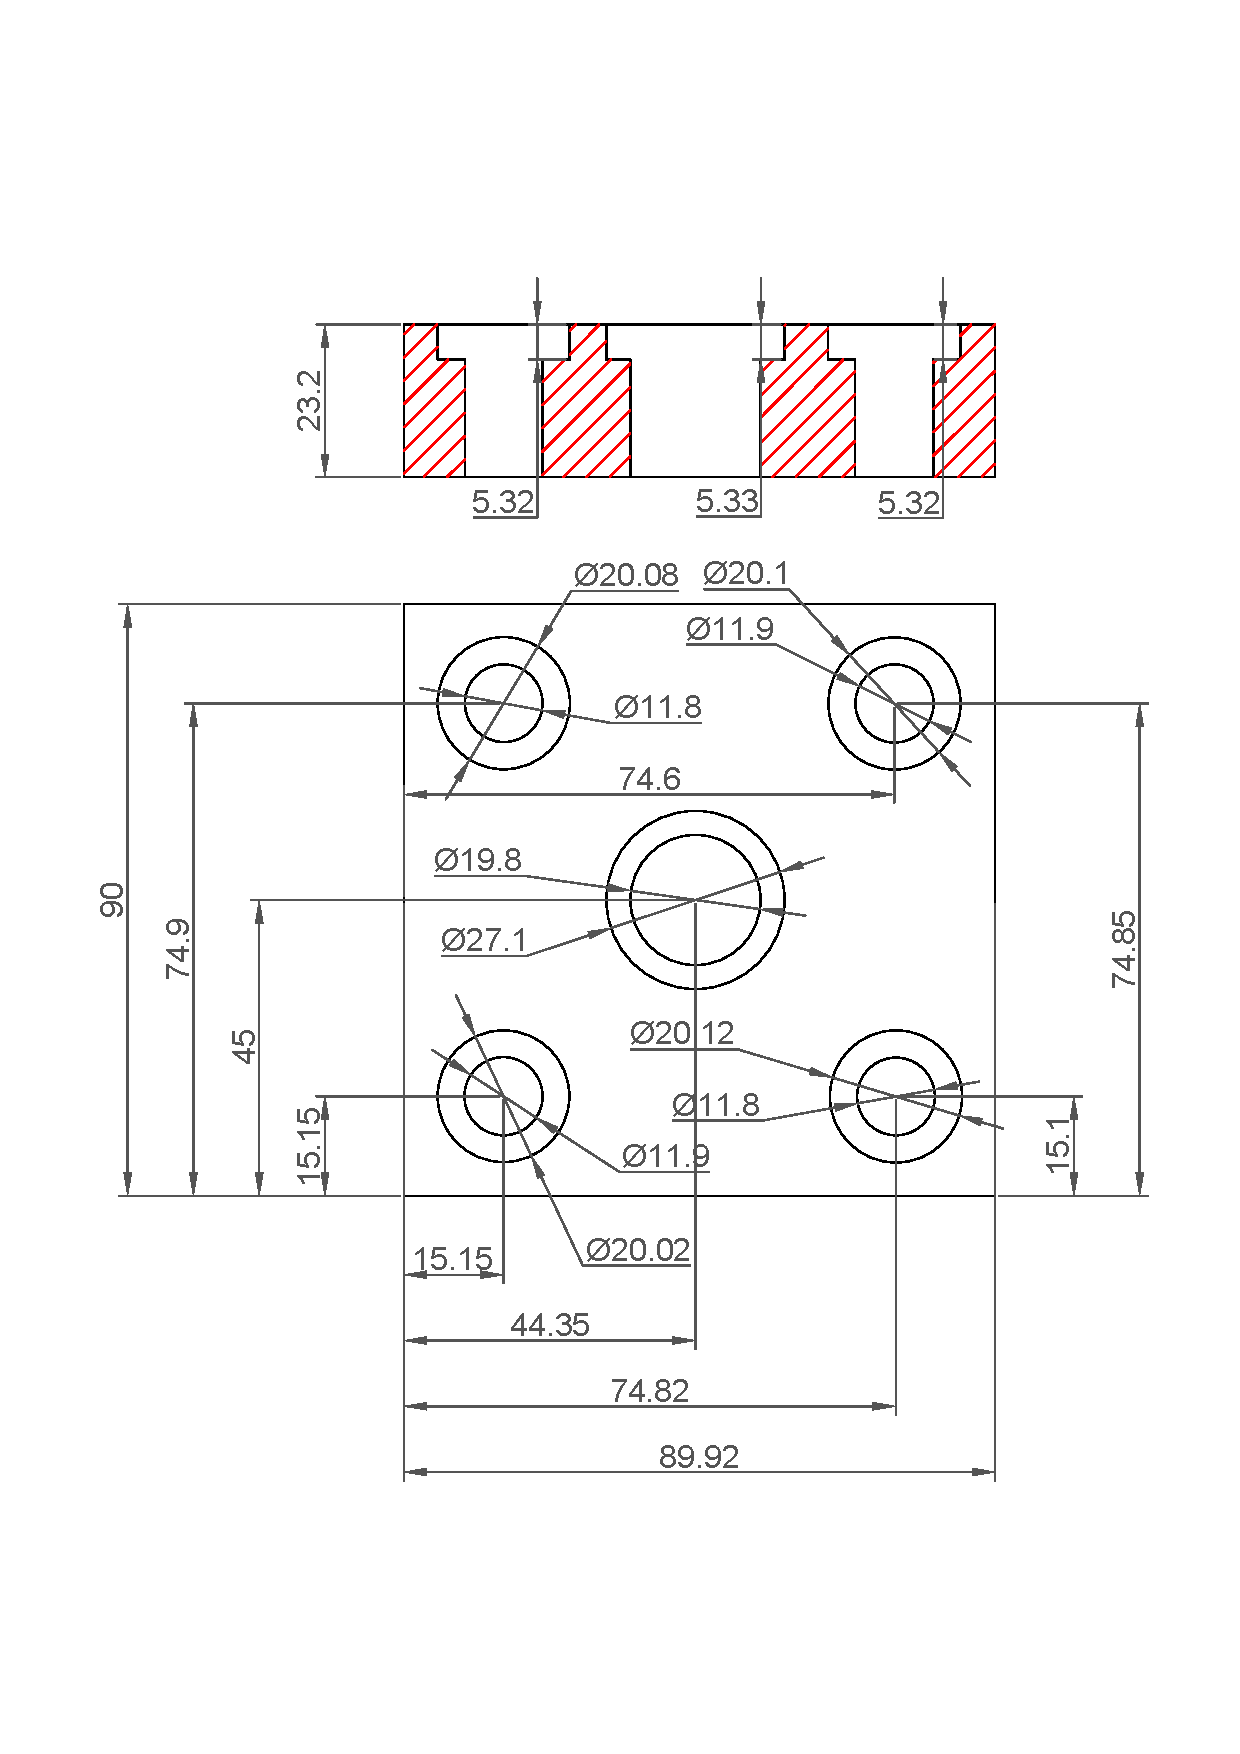
\includegraphics[width=\linewidth]{Meow2.pdf}
	\caption{Kích thước của khối lập phương}
	\label{t}
\end{figure}

